% Options for packages loaded elsewhere
\PassOptionsToPackage{unicode}{hyperref}
\PassOptionsToPackage{hyphens}{url}
%
\documentclass[
]{article}
\usepackage{lmodern}
\usepackage{amsmath}
\usepackage{ifxetex,ifluatex}
\ifnum 0\ifxetex 1\fi\ifluatex 1\fi=0 % if pdftex
  \usepackage[T1]{fontenc}
  \usepackage[utf8]{inputenc}
  \usepackage{textcomp} % provide euro and other symbols
  \usepackage{amssymb}
\else % if luatex or xetex
  \usepackage{unicode-math}
  \defaultfontfeatures{Scale=MatchLowercase}
  \defaultfontfeatures[\rmfamily]{Ligatures=TeX,Scale=1}
\fi
% Use upquote if available, for straight quotes in verbatim environments
\IfFileExists{upquote.sty}{\usepackage{upquote}}{}
\IfFileExists{microtype.sty}{% use microtype if available
  \usepackage[]{microtype}
  \UseMicrotypeSet[protrusion]{basicmath} % disable protrusion for tt fonts
}{}
\makeatletter
\@ifundefined{KOMAClassName}{% if non-KOMA class
  \IfFileExists{parskip.sty}{%
    \usepackage{parskip}
  }{% else
    \setlength{\parindent}{0pt}
    \setlength{\parskip}{6pt plus 2pt minus 1pt}}
}{% if KOMA class
  \KOMAoptions{parskip=half}}
\makeatother
\usepackage{xcolor}
\IfFileExists{xurl.sty}{\usepackage{xurl}}{} % add URL line breaks if available
\IfFileExists{bookmark.sty}{\usepackage{bookmark}}{\usepackage{hyperref}}
\hypersetup{
  pdftitle={Tegaderm CHG IV Securement Dressing for Central Venous and Arterial Catheter Insertion Sites},
  pdfauthor={Andrew J. Sims},
  hidelinks,
  pdfcreator={LaTeX via pandoc}}
\urlstyle{same} % disable monospaced font for URLs
\usepackage[margin=1in]{geometry}
\usepackage{color}
\usepackage{fancyvrb}
\newcommand{\VerbBar}{|}
\newcommand{\VERB}{\Verb[commandchars=\\\{\}]}
\DefineVerbatimEnvironment{Highlighting}{Verbatim}{commandchars=\\\{\}}
% Add ',fontsize=\small' for more characters per line
\usepackage{framed}
\definecolor{shadecolor}{RGB}{248,248,248}
\newenvironment{Shaded}{\begin{snugshade}}{\end{snugshade}}
\newcommand{\AlertTok}[1]{\textcolor[rgb]{0.94,0.16,0.16}{#1}}
\newcommand{\AnnotationTok}[1]{\textcolor[rgb]{0.56,0.35,0.01}{\textbf{\textit{#1}}}}
\newcommand{\AttributeTok}[1]{\textcolor[rgb]{0.77,0.63,0.00}{#1}}
\newcommand{\BaseNTok}[1]{\textcolor[rgb]{0.00,0.00,0.81}{#1}}
\newcommand{\BuiltInTok}[1]{#1}
\newcommand{\CharTok}[1]{\textcolor[rgb]{0.31,0.60,0.02}{#1}}
\newcommand{\CommentTok}[1]{\textcolor[rgb]{0.56,0.35,0.01}{\textit{#1}}}
\newcommand{\CommentVarTok}[1]{\textcolor[rgb]{0.56,0.35,0.01}{\textbf{\textit{#1}}}}
\newcommand{\ConstantTok}[1]{\textcolor[rgb]{0.00,0.00,0.00}{#1}}
\newcommand{\ControlFlowTok}[1]{\textcolor[rgb]{0.13,0.29,0.53}{\textbf{#1}}}
\newcommand{\DataTypeTok}[1]{\textcolor[rgb]{0.13,0.29,0.53}{#1}}
\newcommand{\DecValTok}[1]{\textcolor[rgb]{0.00,0.00,0.81}{#1}}
\newcommand{\DocumentationTok}[1]{\textcolor[rgb]{0.56,0.35,0.01}{\textbf{\textit{#1}}}}
\newcommand{\ErrorTok}[1]{\textcolor[rgb]{0.64,0.00,0.00}{\textbf{#1}}}
\newcommand{\ExtensionTok}[1]{#1}
\newcommand{\FloatTok}[1]{\textcolor[rgb]{0.00,0.00,0.81}{#1}}
\newcommand{\FunctionTok}[1]{\textcolor[rgb]{0.00,0.00,0.00}{#1}}
\newcommand{\ImportTok}[1]{#1}
\newcommand{\InformationTok}[1]{\textcolor[rgb]{0.56,0.35,0.01}{\textbf{\textit{#1}}}}
\newcommand{\KeywordTok}[1]{\textcolor[rgb]{0.13,0.29,0.53}{\textbf{#1}}}
\newcommand{\NormalTok}[1]{#1}
\newcommand{\OperatorTok}[1]{\textcolor[rgb]{0.81,0.36,0.00}{\textbf{#1}}}
\newcommand{\OtherTok}[1]{\textcolor[rgb]{0.56,0.35,0.01}{#1}}
\newcommand{\PreprocessorTok}[1]{\textcolor[rgb]{0.56,0.35,0.01}{\textit{#1}}}
\newcommand{\RegionMarkerTok}[1]{#1}
\newcommand{\SpecialCharTok}[1]{\textcolor[rgb]{0.00,0.00,0.00}{#1}}
\newcommand{\SpecialStringTok}[1]{\textcolor[rgb]{0.31,0.60,0.02}{#1}}
\newcommand{\StringTok}[1]{\textcolor[rgb]{0.31,0.60,0.02}{#1}}
\newcommand{\VariableTok}[1]{\textcolor[rgb]{0.00,0.00,0.00}{#1}}
\newcommand{\VerbatimStringTok}[1]{\textcolor[rgb]{0.31,0.60,0.02}{#1}}
\newcommand{\WarningTok}[1]{\textcolor[rgb]{0.56,0.35,0.01}{\textbf{\textit{#1}}}}
\usepackage{longtable,booktabs}
\usepackage{calc} % for calculating minipage widths
% Correct order of tables after \paragraph or \subparagraph
\usepackage{etoolbox}
\makeatletter
\patchcmd\longtable{\par}{\if@noskipsec\mbox{}\fi\par}{}{}
\makeatother
% Allow footnotes in longtable head/foot
\IfFileExists{footnotehyper.sty}{\usepackage{footnotehyper}}{\usepackage{footnote}}
\makesavenoteenv{longtable}
\usepackage{graphicx}
\makeatletter
\def\maxwidth{\ifdim\Gin@nat@width>\linewidth\linewidth\else\Gin@nat@width\fi}
\def\maxheight{\ifdim\Gin@nat@height>\textheight\textheight\else\Gin@nat@height\fi}
\makeatother
% Scale images if necessary, so that they will not overflow the page
% margins by default, and it is still possible to overwrite the defaults
% using explicit options in \includegraphics[width, height, ...]{}
\setkeys{Gin}{width=\maxwidth,height=\maxheight,keepaspectratio}
% Set default figure placement to htbp
\makeatletter
\def\fps@figure{htbp}
\makeatother
\setlength{\emergencystretch}{3em} % prevent overfull lines
\providecommand{\tightlist}{%
  \setlength{\itemsep}{0pt}\setlength{\parskip}{0pt}}
\setcounter{secnumdepth}{-\maxdimen} % remove section numbering
\ifluatex
  \usepackage{selnolig}  % disable illegal ligatures
\fi
\newlength{\cslhangindent}
\setlength{\cslhangindent}{1.5em}
\newlength{\csllabelwidth}
\setlength{\csllabelwidth}{3em}
\newenvironment{CSLReferences}[2] % #1 hanging-ident, #2 entry spacing
 {% don't indent paragraphs
  \setlength{\parindent}{0pt}
  % turn on hanging indent if param 1 is 1
  \ifodd #1 \everypar{\setlength{\hangindent}{\cslhangindent}}\ignorespaces\fi
  % set entry spacing
  \ifnum #2 > 0
  \setlength{\parskip}{#2\baselineskip}
  \fi
 }%
 {}
\usepackage{calc}
\newcommand{\CSLBlock}[1]{#1\hfill\break}
\newcommand{\CSLLeftMargin}[1]{\parbox[t]{\csllabelwidth}{#1}}
\newcommand{\CSLRightInline}[1]{\parbox[t]{\linewidth - \csllabelwidth}{#1}\break}
\newcommand{\CSLIndent}[1]{\hspace{\cslhangindent}#1}

\title{Tegaderm CHG IV Securement Dressing for Central Venous and
Arterial Catheter Insertion Sites}
\usepackage{etoolbox}
\makeatletter
\providecommand{\subtitle}[1]{% add subtitle to \maketitle
  \apptocmd{\@title}{\par {\large #1 \par}}{}{}
}
\makeatother
\subtitle{A decision tree example with probabilistic sensitivity
analysis}
\author{Andrew J. Sims}
\date{July 2020}

\begin{document}
\maketitle

\hypertarget{introduction}{%
\section{Introduction}\label{introduction}}

This vignette is an example of modelling a decision tree using the
\texttt{rdecision} package, with probabilistic sensitivity analysis. It
is based on the model reported by Jenks \emph{et al} {[}1{]} in which a
transparent dressing used to secure vascular catheters (Tegaderm CHG)
was compared with a standard dressing.

\hypertarget{model-variables}{%
\section{Model variables}\label{model-variables}}

Thirteen variables were used in the model. The choice of variables,
their distributions and their parameters are taken from table 3 of Jenks
\emph{et al} {[}1{]}, with the following additional information:

\begin{itemize}
\tightlist
\item
  For variables with lognormal uncertainty, the manufacturer synthesized
  a log normal distribution as \(\exp(\alpha + \beta r())\) where
  \(r()\) is a random draw from a standard normal distribution. This
  does not follow the parametrizations of the LogNormModVar provided in
  \texttt{rdecision}, but can be reproduced using expression model
  variables. Three standard normal model variables were introduced for
  this purpose.
\item
  The values for \(\alpha\) and \(\beta\) for the hazard ratio for CRBSI
  and LSI were -0.911 and -0.393 respectively, and 1.482 and 0.490 for
  the relative risk of dermatitis.
\item
  The probabilities of CRBSI and LSI for standard dressings (\(p\)) were
  modified by the hazard ratio for Tegaderm using the form
  \((1-(1-p)^h)\) where \(h\) is the hazard ratio. Relative risks were
  applied as multipliers.
\item
  The point estimate cost of CRBSI was £9900, not £9990, although the
  parameters (198,50) are quoted correctly.
\end{itemize}

The model variables were constructed as follows:

\begin{Shaded}
\begin{Highlighting}[]
\CommentTok{\# standard normals}
\NormalTok{n1 }\OtherTok{\textless{}{-}}\NormalTok{ NormModVar}\SpecialCharTok{$}\FunctionTok{new}\NormalTok{(}\StringTok{"SN1"}\NormalTok{,}\StringTok{""}\NormalTok{, }\DecValTok{0}\NormalTok{, }\DecValTok{1}\NormalTok{)}
\NormalTok{n2 }\OtherTok{\textless{}{-}}\NormalTok{ NormModVar}\SpecialCharTok{$}\FunctionTok{new}\NormalTok{(}\StringTok{"SN2"}\NormalTok{,}\StringTok{""}\NormalTok{, }\DecValTok{0}\NormalTok{, }\DecValTok{1}\NormalTok{)}
\NormalTok{n3 }\OtherTok{\textless{}{-}}\NormalTok{ NormModVar}\SpecialCharTok{$}\FunctionTok{new}\NormalTok{(}\StringTok{"SN3"}\NormalTok{,}\StringTok{""}\NormalTok{, }\DecValTok{0}\NormalTok{, }\DecValTok{1}\NormalTok{)}
  
\CommentTok{\# clinical variables}
\NormalTok{r.CRBSI }\OtherTok{\textless{}{-}}\NormalTok{ NormModVar}\SpecialCharTok{$}\FunctionTok{new}\NormalTok{(}
  \StringTok{\textquotesingle{}Baseline CRBSI rate\textquotesingle{}}\NormalTok{, }\StringTok{\textquotesingle{}/1000 catheter days\textquotesingle{}}\NormalTok{, }\AttributeTok{mu=}\FloatTok{1.48}\NormalTok{, }\AttributeTok{sigma=}\FloatTok{0.074}
\NormalTok{)}
\NormalTok{hr.CRBSI }\OtherTok{\textless{}{-}}\NormalTok{ ExprModVar}\SpecialCharTok{$}\FunctionTok{new}\NormalTok{(}
  \StringTok{"Tegaderm CRBSI HR"}\NormalTok{, }
  \StringTok{"HR"}\NormalTok{, }
\NormalTok{  rlang}\SpecialCharTok{::}\FunctionTok{quo}\NormalTok{(}\FunctionTok{exp}\NormalTok{(}\SpecialCharTok{{-}}\FloatTok{0.911{-}0.393}\SpecialCharTok{*}\NormalTok{n1))}
\NormalTok{)}
\NormalTok{hr.LSI }\OtherTok{\textless{}{-}}\NormalTok{ ExprModVar}\SpecialCharTok{$}\FunctionTok{new}\NormalTok{(}
  \StringTok{"Tegaderm LSI HR"}\NormalTok{, }
  \StringTok{"HR"}\NormalTok{, }
\NormalTok{  rlang}\SpecialCharTok{::}\FunctionTok{quo}\NormalTok{(}\FunctionTok{exp}\NormalTok{(}\SpecialCharTok{{-}}\FloatTok{0.911{-}0.393}\SpecialCharTok{*}\NormalTok{n2))}
\NormalTok{)}
\NormalTok{r.Dermatitis }\OtherTok{\textless{}{-}}\NormalTok{ NormModVar}\SpecialCharTok{$}\FunctionTok{new}\NormalTok{(}
  \StringTok{\textquotesingle{}Baseline dermatitis risk\textquotesingle{}}\NormalTok{, }\StringTok{\textquotesingle{}/catheter\textquotesingle{}}\NormalTok{, }\AttributeTok{mu=}\FloatTok{0.0026}\NormalTok{, }\AttributeTok{sigma=}\FloatTok{0.00026}
\NormalTok{)}
\NormalTok{rr.Dermatitis }\OtherTok{\textless{}{-}}\NormalTok{ ExprModVar}\SpecialCharTok{$}\FunctionTok{new}\NormalTok{(}
  \StringTok{"Tegaderm LSI HR"}\NormalTok{, }
  \StringTok{"HR"}\NormalTok{, }
\NormalTok{  rlang}\SpecialCharTok{::}\FunctionTok{quo}\NormalTok{(}\FunctionTok{exp}\NormalTok{(}\FloatTok{1.482{-}0.490}\SpecialCharTok{*}\NormalTok{n3))}
\NormalTok{)}

\CommentTok{\# cost variables}
\NormalTok{c.CRBSI }\OtherTok{\textless{}{-}}\NormalTok{ GammaModVar}\SpecialCharTok{$}\FunctionTok{new}\NormalTok{(}
  \StringTok{\textquotesingle{}CRBSI cost\textquotesingle{}}\NormalTok{, }\StringTok{\textquotesingle{}GBP\textquotesingle{}}\NormalTok{, }\AttributeTok{shape=}\FloatTok{198.0}\NormalTok{, }\AttributeTok{scale=}\DecValTok{50}
\NormalTok{)}
\NormalTok{c.Dermatitis }\OtherTok{\textless{}{-}}\NormalTok{ GammaModVar}\SpecialCharTok{$}\FunctionTok{new}\NormalTok{(}
  \StringTok{\textquotesingle{}Dermatitis cost\textquotesingle{}}\NormalTok{, }\StringTok{\textquotesingle{}GBP\textquotesingle{}}\NormalTok{, }\AttributeTok{shape=}\DecValTok{30}\NormalTok{, }\AttributeTok{scale=}\DecValTok{5}
\NormalTok{)}
\NormalTok{c.LSI }\OtherTok{\textless{}{-}}\NormalTok{ GammaModVar}\SpecialCharTok{$}\FunctionTok{new}\NormalTok{(}
  \StringTok{\textquotesingle{}LSI cost\textquotesingle{}}\NormalTok{, }\StringTok{\textquotesingle{}GBP\textquotesingle{}}\NormalTok{, }\AttributeTok{shape=}\DecValTok{50}\NormalTok{, }\AttributeTok{scale=}\DecValTok{5}
\NormalTok{)}
\NormalTok{n.catheters }\OtherTok{\textless{}{-}}\NormalTok{ NormModVar}\SpecialCharTok{$}\FunctionTok{new}\NormalTok{(}
  \StringTok{\textquotesingle{}No. catheters\textquotesingle{}}\NormalTok{, }\StringTok{\textquotesingle{}catheters\textquotesingle{}}\NormalTok{, }\AttributeTok{mu=}\DecValTok{3}\NormalTok{, }\AttributeTok{sigma=}\FloatTok{0.3} 
\NormalTok{)}
\NormalTok{c.Tegaderm }\OtherTok{\textless{}{-}}\NormalTok{ ExprModVar}\SpecialCharTok{$}\FunctionTok{new}\NormalTok{(}
  \StringTok{"Tegaderm CHG cost"}\NormalTok{, }\StringTok{"GBP"}\NormalTok{, rlang}\SpecialCharTok{::}\FunctionTok{quo}\NormalTok{(}\FloatTok{6.21}\SpecialCharTok{*}\NormalTok{n.catheters)}
\NormalTok{)}
\NormalTok{c.Standard }\OtherTok{\textless{}{-}}\NormalTok{ ExprModVar}\SpecialCharTok{$}\FunctionTok{new}\NormalTok{(}
  \StringTok{"Standard dressing cost"}\NormalTok{, }\StringTok{"GBP"}\NormalTok{, rlang}\SpecialCharTok{::}\FunctionTok{quo}\NormalTok{(}\FloatTok{1.34}\SpecialCharTok{*}\NormalTok{n.catheters)}
\NormalTok{)}
\NormalTok{n.cathdays }\OtherTok{\textless{}{-}}\NormalTok{ NormModVar}\SpecialCharTok{$}\FunctionTok{new}\NormalTok{(}
  \StringTok{\textquotesingle{}No. days with catheter\textquotesingle{}}\NormalTok{, }\StringTok{\textquotesingle{}days\textquotesingle{}}\NormalTok{, }\AttributeTok{mu=}\DecValTok{10}\NormalTok{, }\AttributeTok{sigma=}\DecValTok{2}
\NormalTok{)  }
\end{Highlighting}
\end{Shaded}

\hypertarget{model-variable-expressions}{%
\section{Model variable expressions}\label{model-variable-expressions}}

Variables in the model may be included in the decision tree via
mathematical expressions, which involve model variables and are
themselves model variables. Forms of expression involving R's numerical
functions and multiple model variables are supported, provided they
conform to R syntax. The following code creates the model variable
expressions to be used as values in the decision tree edges. For
probabilities, the convention \(q = 1-p\) is used to ensure that the sum
of probabilities leaving each chance node sums to one.

\begin{Shaded}
\begin{Highlighting}[]
\CommentTok{\# probabilities}
\NormalTok{p.Dermatitis.S }\OtherTok{\textless{}{-}}\NormalTok{ ExprModVar}\SpecialCharTok{$}\FunctionTok{new}\NormalTok{(}
  \StringTok{\textquotesingle{}P(dermatitis|standard dressing)\textquotesingle{}}\NormalTok{, }\StringTok{\textquotesingle{}P\textquotesingle{}}\NormalTok{, }
\NormalTok{  rlang}\SpecialCharTok{::}\FunctionTok{quo}\NormalTok{(r.Dermatitis}\SpecialCharTok{*}\NormalTok{n.catheters)}
\NormalTok{)}
\NormalTok{q.Dermatitis.S }\OtherTok{\textless{}{-}}\NormalTok{ ExprModVar}\SpecialCharTok{$}\FunctionTok{new}\NormalTok{(}
  \StringTok{\textquotesingle{}Q(dermatitis|standard dressing)\textquotesingle{}}\NormalTok{, }\StringTok{\textquotesingle{}1{-}P\textquotesingle{}}\NormalTok{, }
\NormalTok{  rlang}\SpecialCharTok{::}\FunctionTok{quo}\NormalTok{(}\DecValTok{1}\SpecialCharTok{{-}}\NormalTok{p.Dermatitis.S)}
\NormalTok{)}
\NormalTok{p.Dermatitis.T }\OtherTok{\textless{}{-}}\NormalTok{ ExprModVar}\SpecialCharTok{$}\FunctionTok{new}\NormalTok{(}
  \StringTok{\textquotesingle{}P(dermatitis|Tegaderm)\textquotesingle{}}\NormalTok{, }\StringTok{\textquotesingle{}P\textquotesingle{}}\NormalTok{, }
\NormalTok{  rlang}\SpecialCharTok{::}\FunctionTok{quo}\NormalTok{(r.Dermatitis}\SpecialCharTok{*}\NormalTok{rr.Dermatitis}\SpecialCharTok{*}\NormalTok{n.catheters)}
\NormalTok{)}
\NormalTok{q.Dermatitis.T }\OtherTok{\textless{}{-}}\NormalTok{ ExprModVar}\SpecialCharTok{$}\FunctionTok{new}\NormalTok{(}
  \StringTok{\textquotesingle{}Q(dermatitis|Tegaderm)\textquotesingle{}}\NormalTok{, }\StringTok{\textquotesingle{}1{-}P\textquotesingle{}}\NormalTok{, }
\NormalTok{  rlang}\SpecialCharTok{::}\FunctionTok{quo}\NormalTok{(}\DecValTok{1}\SpecialCharTok{{-}}\NormalTok{p.Dermatitis.T)}
\NormalTok{)}

\NormalTok{p.LSI.S }\OtherTok{\textless{}{-}}\NormalTok{ NormModVar}\SpecialCharTok{$}\FunctionTok{new}\NormalTok{(}
  \StringTok{\textquotesingle{}P(LSI|Standard)\textquotesingle{}}\NormalTok{, }\StringTok{\textquotesingle{}/patient\textquotesingle{}}\NormalTok{, }\AttributeTok{mu=}\FloatTok{0.1}\NormalTok{, }\AttributeTok{sigma=}\FloatTok{0.01} 
\NormalTok{)}
\NormalTok{q.LSI.S }\OtherTok{\textless{}{-}}\NormalTok{ ExprModVar}\SpecialCharTok{$}\FunctionTok{new}\NormalTok{(}
  \StringTok{\textquotesingle{}Q(LSI|Standard)\textquotesingle{}}\NormalTok{, }\StringTok{\textquotesingle{}1{-}P\textquotesingle{}}\NormalTok{, rlang}\SpecialCharTok{::}\FunctionTok{quo}\NormalTok{(}\DecValTok{1}\SpecialCharTok{{-}}\NormalTok{p.LSI.S) }
\NormalTok{)}
\NormalTok{p.LSI.T }\OtherTok{\textless{}{-}}\NormalTok{ ExprModVar}\SpecialCharTok{$}\FunctionTok{new}\NormalTok{(}
  \StringTok{\textquotesingle{}P(LSI|Tegaderm)\textquotesingle{}}\NormalTok{, }\StringTok{\textquotesingle{}P\textquotesingle{}}\NormalTok{, rlang}\SpecialCharTok{::}\FunctionTok{quo}\NormalTok{(}\DecValTok{1}\SpecialCharTok{{-}}\NormalTok{(}\DecValTok{1}\SpecialCharTok{{-}}\NormalTok{p.LSI.S)}\SpecialCharTok{\^{}}\NormalTok{hr.LSI)}
\NormalTok{)}
\NormalTok{q.LSI.T }\OtherTok{\textless{}{-}}\NormalTok{ ExprModVar}\SpecialCharTok{$}\FunctionTok{new}\NormalTok{(}
  \StringTok{\textquotesingle{}Q(LSI|Tegaderm)\textquotesingle{}}\NormalTok{, }\StringTok{\textquotesingle{}1{-}P\textquotesingle{}}\NormalTok{, rlang}\SpecialCharTok{::}\FunctionTok{quo}\NormalTok{(}\DecValTok{1}\SpecialCharTok{{-}}\NormalTok{p.LSI.T)}
\NormalTok{)}

\NormalTok{p.CRBSI.S }\OtherTok{\textless{}{-}}\NormalTok{ ExprModVar}\SpecialCharTok{$}\FunctionTok{new}\NormalTok{(}
  \StringTok{\textquotesingle{}P(CRBSI|standard dressing)\textquotesingle{}}\NormalTok{, }\StringTok{\textquotesingle{}P\textquotesingle{}}\NormalTok{,  rlang}\SpecialCharTok{::}\FunctionTok{quo}\NormalTok{(r.CRBSI}\SpecialCharTok{*}\NormalTok{n.cathdays}\SpecialCharTok{/}\DecValTok{1000}\NormalTok{)}
\NormalTok{)}
\NormalTok{q.CRBSI.S }\OtherTok{\textless{}{-}}\NormalTok{ ExprModVar}\SpecialCharTok{$}\FunctionTok{new}\NormalTok{(}
  \StringTok{\textquotesingle{}Q(CRBSI|standard dressing)\textquotesingle{}}\NormalTok{, }\StringTok{\textquotesingle{}1{-}P\textquotesingle{}}\NormalTok{,  rlang}\SpecialCharTok{::}\FunctionTok{quo}\NormalTok{(}\DecValTok{1}\SpecialCharTok{{-}}\NormalTok{p.CRBSI.S)}
\NormalTok{)}
\NormalTok{p.CRBSI.T }\OtherTok{\textless{}{-}}\NormalTok{ ExprModVar}\SpecialCharTok{$}\FunctionTok{new}\NormalTok{(}
  \StringTok{\textquotesingle{}P(CRBSI|Tegaderm)\textquotesingle{}}\NormalTok{, }\StringTok{\textquotesingle{}P\textquotesingle{}}\NormalTok{, rlang}\SpecialCharTok{::}\FunctionTok{quo}\NormalTok{(}\DecValTok{1}\SpecialCharTok{{-}}\NormalTok{(}\DecValTok{1}\SpecialCharTok{{-}}\NormalTok{r.CRBSI}\SpecialCharTok{*}\NormalTok{n.cathdays}\SpecialCharTok{/}\DecValTok{1000}\NormalTok{)}\SpecialCharTok{\^{}}\NormalTok{hr.CRBSI)}
\NormalTok{)}
\NormalTok{q.CRBSI.T }\OtherTok{\textless{}{-}}\NormalTok{ ExprModVar}\SpecialCharTok{$}\FunctionTok{new}\NormalTok{(}
  \StringTok{\textquotesingle{}Q(CRBSI|Tegaderm)\textquotesingle{}}\NormalTok{, }\StringTok{\textquotesingle{}1{-}P\textquotesingle{}}\NormalTok{, rlang}\SpecialCharTok{::}\FunctionTok{quo}\NormalTok{(}\DecValTok{1}\SpecialCharTok{{-}}\NormalTok{p.CRBSI.T)}
\NormalTok{)}
\end{Highlighting}
\end{Shaded}

\hypertarget{the-decision-tree}{%
\section{The decision tree}\label{the-decision-tree}}

The following code constructs the decision tree based on figure 2 of
Jenks \emph{et al} {[}1{]}. In the formulation used by
\texttt{rdecision}, the decision tree is constructed from sets of
decision, chance and leaf nodes and from edges (actions and reactions).
Leaf nodes are synonymous with pathways in Briggs' terminology {[}2{]}.
The time horizon is not stated explicitly in the model, and is assumed
to be 7 days. It was implied that the time horizon was ICU stay plus
some follow-up, and the costs reflect those incurred in that period, so
the assumption of 7 days does not affect the \texttt{rdecision}
implementation of the model.

The tree is somewhat more complex than figure 2 of Jenks \emph{et al}
because it allows for patients to have more than one adverse event (AE)
during their stay (whereas figure 2 implies that only one event per
patient is possible). The rates of AE were estimated independently, and
allow for multiple events.

\begin{Shaded}
\begin{Highlighting}[]
\CommentTok{\# create decision tree}
\NormalTok{th }\OtherTok{\textless{}{-}} \FunctionTok{as.difftime}\NormalTok{(}\DecValTok{7}\NormalTok{, }\AttributeTok{units=}\StringTok{"days"}\NormalTok{)}
\CommentTok{\# standard dressing}
\NormalTok{t01 }\OtherTok{\textless{}{-}}\NormalTok{ LeafNode}\SpecialCharTok{$}\FunctionTok{new}\NormalTok{(}\StringTok{"t01"}\NormalTok{, }\AttributeTok{interval=}\NormalTok{th)}
\NormalTok{t02 }\OtherTok{\textless{}{-}}\NormalTok{ LeafNode}\SpecialCharTok{$}\FunctionTok{new}\NormalTok{(}\StringTok{"t02"}\NormalTok{, }\AttributeTok{interval=}\NormalTok{th)}
\NormalTok{c01 }\OtherTok{\textless{}{-}}\NormalTok{ ChanceNode}\SpecialCharTok{$}\FunctionTok{new}\NormalTok{()}
\NormalTok{e01 }\OtherTok{\textless{}{-}}\NormalTok{ Reaction}\SpecialCharTok{$}\FunctionTok{new}\NormalTok{(c01,t01,}\AttributeTok{p=}\NormalTok{p.Dermatitis.S,}\AttributeTok{cost=}\NormalTok{c.Dermatitis,}
                    \AttributeTok{label=}\StringTok{"Dermatitis"}\NormalTok{)}
\NormalTok{e02 }\OtherTok{\textless{}{-}}\NormalTok{ Reaction}\SpecialCharTok{$}\FunctionTok{new}\NormalTok{(c01,t02,}\AttributeTok{p=}\NormalTok{q.Dermatitis.S,}\AttributeTok{cost=}\DecValTok{0}\NormalTok{,}
                    \AttributeTok{label=}\StringTok{"No dermatitis"}\NormalTok{)}
\CommentTok{\#}
\NormalTok{t03 }\OtherTok{\textless{}{-}}\NormalTok{ LeafNode}\SpecialCharTok{$}\FunctionTok{new}\NormalTok{(}\StringTok{"t03"}\NormalTok{, }\AttributeTok{interval=}\NormalTok{th)}
\NormalTok{t04 }\OtherTok{\textless{}{-}}\NormalTok{ LeafNode}\SpecialCharTok{$}\FunctionTok{new}\NormalTok{(}\StringTok{"t04"}\NormalTok{, }\AttributeTok{interval=}\NormalTok{th)}
\NormalTok{c02 }\OtherTok{\textless{}{-}}\NormalTok{ ChanceNode}\SpecialCharTok{$}\FunctionTok{new}\NormalTok{()}
\NormalTok{e03 }\OtherTok{\textless{}{-}}\NormalTok{ Reaction}\SpecialCharTok{$}\FunctionTok{new}\NormalTok{(c02,t03,}\AttributeTok{p=}\NormalTok{p.Dermatitis.S,}\AttributeTok{cost=}\NormalTok{c.Dermatitis,}
                    \AttributeTok{label=}\StringTok{"Dermatitis"}\NormalTok{)}
\NormalTok{e04 }\OtherTok{\textless{}{-}}\NormalTok{ Reaction}\SpecialCharTok{$}\FunctionTok{new}\NormalTok{(c02,t04,}\AttributeTok{p=}\NormalTok{q.Dermatitis.S,}\AttributeTok{cost=}\DecValTok{0}\NormalTok{,}
                    \AttributeTok{label=}\StringTok{"No dermatitis"}\NormalTok{)}
\CommentTok{\#}
\NormalTok{c03 }\OtherTok{\textless{}{-}}\NormalTok{ ChanceNode}\SpecialCharTok{$}\FunctionTok{new}\NormalTok{()}
\NormalTok{e05 }\OtherTok{\textless{}{-}}\NormalTok{ Reaction}\SpecialCharTok{$}\FunctionTok{new}\NormalTok{(c03,c01,}\AttributeTok{p=}\NormalTok{p.LSI.S,}\AttributeTok{cost=}\NormalTok{c.LSI,}\AttributeTok{label=}\StringTok{"LSI"}\NormalTok{)}
\NormalTok{e06 }\OtherTok{\textless{}{-}}\NormalTok{ Reaction}\SpecialCharTok{$}\FunctionTok{new}\NormalTok{(c03,c02,}\AttributeTok{p=}\NormalTok{q.LSI.S,}\AttributeTok{cost=}\DecValTok{0}\NormalTok{,}\AttributeTok{label=}\StringTok{"No LSI"}\NormalTok{)}
\CommentTok{\#}
\NormalTok{t11 }\OtherTok{\textless{}{-}}\NormalTok{ LeafNode}\SpecialCharTok{$}\FunctionTok{new}\NormalTok{(}\StringTok{"t11"}\NormalTok{, }\AttributeTok{interval=}\NormalTok{th)}
\NormalTok{t12 }\OtherTok{\textless{}{-}}\NormalTok{ LeafNode}\SpecialCharTok{$}\FunctionTok{new}\NormalTok{(}\StringTok{"t12"}\NormalTok{, }\AttributeTok{interval=}\NormalTok{th)}
\NormalTok{c11 }\OtherTok{\textless{}{-}}\NormalTok{ ChanceNode}\SpecialCharTok{$}\FunctionTok{new}\NormalTok{()}
\NormalTok{e11 }\OtherTok{\textless{}{-}}\NormalTok{ Reaction}\SpecialCharTok{$}\FunctionTok{new}\NormalTok{(c11,t11,}\AttributeTok{p=}\NormalTok{p.Dermatitis.S,}\AttributeTok{cost=}\NormalTok{c.Dermatitis,}
                    \AttributeTok{label=}\StringTok{"Dermatitis"}\NormalTok{)}
\NormalTok{e12 }\OtherTok{\textless{}{-}}\NormalTok{ Reaction}\SpecialCharTok{$}\FunctionTok{new}\NormalTok{(c11,t12,}\AttributeTok{p=}\NormalTok{q.Dermatitis.S,}\AttributeTok{cost=}\DecValTok{0}\NormalTok{,}\AttributeTok{label=}\StringTok{"No Dermatitis"}\NormalTok{)}
\CommentTok{\#}
\NormalTok{t13 }\OtherTok{\textless{}{-}}\NormalTok{ LeafNode}\SpecialCharTok{$}\FunctionTok{new}\NormalTok{(}\StringTok{"t13"}\NormalTok{, }\AttributeTok{interval=}\NormalTok{th)}
\NormalTok{t14 }\OtherTok{\textless{}{-}}\NormalTok{ LeafNode}\SpecialCharTok{$}\FunctionTok{new}\NormalTok{(}\StringTok{"t14"}\NormalTok{, }\AttributeTok{interval=}\NormalTok{th)}
\NormalTok{c12 }\OtherTok{\textless{}{-}}\NormalTok{ ChanceNode}\SpecialCharTok{$}\FunctionTok{new}\NormalTok{()}
\NormalTok{e13 }\OtherTok{\textless{}{-}}\NormalTok{ Reaction}\SpecialCharTok{$}\FunctionTok{new}\NormalTok{(c12,t13,}\AttributeTok{p=}\NormalTok{p.Dermatitis.S,}\AttributeTok{cost=}\NormalTok{c.Dermatitis, }
                    \AttributeTok{label=}\StringTok{"Dermatitis"}\NormalTok{)}
\NormalTok{e14 }\OtherTok{\textless{}{-}}\NormalTok{ Reaction}\SpecialCharTok{$}\FunctionTok{new}\NormalTok{(c12,t14,}\AttributeTok{p=}\NormalTok{q.Dermatitis.S,}\AttributeTok{cost=}\DecValTok{0}\NormalTok{,}\AttributeTok{label=}\StringTok{"No dermatitis"}\NormalTok{)}
\CommentTok{\#}
\NormalTok{c13 }\OtherTok{\textless{}{-}}\NormalTok{ ChanceNode}\SpecialCharTok{$}\FunctionTok{new}\NormalTok{()}
\NormalTok{e15 }\OtherTok{\textless{}{-}}\NormalTok{ Reaction}\SpecialCharTok{$}\FunctionTok{new}\NormalTok{(c13,c11,}\AttributeTok{p=}\NormalTok{p.LSI.S,}\AttributeTok{cost=}\NormalTok{c.LSI,}\AttributeTok{label=}\StringTok{"LSI"}\NormalTok{)}
\NormalTok{e16 }\OtherTok{\textless{}{-}}\NormalTok{ Reaction}\SpecialCharTok{$}\FunctionTok{new}\NormalTok{(c13,c12,}\AttributeTok{p=}\NormalTok{q.LSI.S,}\AttributeTok{cost=}\DecValTok{0}\NormalTok{,}\AttributeTok{label=}\StringTok{"No LSI"}\NormalTok{)}
\CommentTok{\#}
\NormalTok{c23 }\OtherTok{\textless{}{-}}\NormalTok{ ChanceNode}\SpecialCharTok{$}\FunctionTok{new}\NormalTok{()}
\NormalTok{e21 }\OtherTok{\textless{}{-}}\NormalTok{ Reaction}\SpecialCharTok{$}\FunctionTok{new}\NormalTok{(c23,c03,}\AttributeTok{p=}\NormalTok{p.CRBSI.S,}\AttributeTok{cost=}\NormalTok{c.CRBSI,}\AttributeTok{label=}\StringTok{"CRBSI"}\NormalTok{)}
\NormalTok{e22 }\OtherTok{\textless{}{-}}\NormalTok{ Reaction}\SpecialCharTok{$}\FunctionTok{new}\NormalTok{(c23,c13,}\AttributeTok{p=}\NormalTok{q.CRBSI.S,}\AttributeTok{cost=}\DecValTok{0}\NormalTok{,}\AttributeTok{label=}\StringTok{"No CRBSI"}\NormalTok{)}
\CommentTok{\#}
\CommentTok{\# Tegaderm branch  }
\NormalTok{t31 }\OtherTok{\textless{}{-}}\NormalTok{ LeafNode}\SpecialCharTok{$}\FunctionTok{new}\NormalTok{(}\StringTok{"t31"}\NormalTok{, }\AttributeTok{interval=}\NormalTok{th)}
\NormalTok{t32 }\OtherTok{\textless{}{-}}\NormalTok{ LeafNode}\SpecialCharTok{$}\FunctionTok{new}\NormalTok{(}\StringTok{"t32"}\NormalTok{, }\AttributeTok{interval=}\NormalTok{th)}
\NormalTok{c31 }\OtherTok{\textless{}{-}}\NormalTok{ ChanceNode}\SpecialCharTok{$}\FunctionTok{new}\NormalTok{()}
\NormalTok{e31 }\OtherTok{\textless{}{-}}\NormalTok{ Reaction}\SpecialCharTok{$}\FunctionTok{new}\NormalTok{(c31,t31,}\AttributeTok{p=}\NormalTok{p.Dermatitis.T,}\AttributeTok{cost=}\NormalTok{c.Dermatitis,}
                    \AttributeTok{label=}\StringTok{"Dermatitis"}\NormalTok{)}
\NormalTok{e32 }\OtherTok{\textless{}{-}}\NormalTok{ Reaction}\SpecialCharTok{$}\FunctionTok{new}\NormalTok{(c31,t32,}\AttributeTok{p=}\NormalTok{q.Dermatitis.T,}\AttributeTok{cost=}\DecValTok{0}\NormalTok{,}\AttributeTok{label=}\StringTok{"no dermatitis"}\NormalTok{)}
\CommentTok{\#}
\NormalTok{t33 }\OtherTok{\textless{}{-}}\NormalTok{ LeafNode}\SpecialCharTok{$}\FunctionTok{new}\NormalTok{(}\StringTok{"t33"}\NormalTok{, }\AttributeTok{interval=}\NormalTok{th)}
\NormalTok{t34 }\OtherTok{\textless{}{-}}\NormalTok{ LeafNode}\SpecialCharTok{$}\FunctionTok{new}\NormalTok{(}\StringTok{"t34"}\NormalTok{, }\AttributeTok{interval=}\NormalTok{th)}
\NormalTok{c32 }\OtherTok{\textless{}{-}}\NormalTok{ ChanceNode}\SpecialCharTok{$}\FunctionTok{new}\NormalTok{()}
\NormalTok{e33 }\OtherTok{\textless{}{-}}\NormalTok{ Reaction}\SpecialCharTok{$}\FunctionTok{new}\NormalTok{(c32,t33,}\AttributeTok{p=}\NormalTok{p.Dermatitis.T,}\AttributeTok{cost=}\NormalTok{c.Dermatitis,}
                    \AttributeTok{label=}\StringTok{"Dermatitis"}\NormalTok{)}
\NormalTok{e34 }\OtherTok{\textless{}{-}}\NormalTok{ Reaction}\SpecialCharTok{$}\FunctionTok{new}\NormalTok{(c32,t34,}\AttributeTok{p=}\NormalTok{q.Dermatitis.T,}\AttributeTok{cost=}\DecValTok{0}\NormalTok{,}\AttributeTok{label=}\StringTok{"No dermatitis"}\NormalTok{)}
\CommentTok{\#}
\NormalTok{c33 }\OtherTok{\textless{}{-}}\NormalTok{ ChanceNode}\SpecialCharTok{$}\FunctionTok{new}\NormalTok{()}
\NormalTok{e35 }\OtherTok{\textless{}{-}}\NormalTok{ Reaction}\SpecialCharTok{$}\FunctionTok{new}\NormalTok{(c33,c31,}\AttributeTok{p=}\NormalTok{p.LSI.T,}\AttributeTok{cost=}\NormalTok{c.LSI,}\AttributeTok{label=}\StringTok{"LSI"}\NormalTok{)}
\NormalTok{e36 }\OtherTok{\textless{}{-}}\NormalTok{ Reaction}\SpecialCharTok{$}\FunctionTok{new}\NormalTok{(c33,c32,}\AttributeTok{p=}\NormalTok{q.LSI.T,}\AttributeTok{cost=}\DecValTok{0}\NormalTok{,}\AttributeTok{label=}\StringTok{"No LSI"}\NormalTok{)}
\CommentTok{\#}
\NormalTok{t41 }\OtherTok{\textless{}{-}}\NormalTok{ LeafNode}\SpecialCharTok{$}\FunctionTok{new}\NormalTok{(}\StringTok{"t41"}\NormalTok{, }\AttributeTok{interval=}\NormalTok{th)}
\NormalTok{t42 }\OtherTok{\textless{}{-}}\NormalTok{ LeafNode}\SpecialCharTok{$}\FunctionTok{new}\NormalTok{(}\StringTok{"t42"}\NormalTok{, }\AttributeTok{interval=}\NormalTok{th)}
\NormalTok{c41 }\OtherTok{\textless{}{-}}\NormalTok{ ChanceNode}\SpecialCharTok{$}\FunctionTok{new}\NormalTok{()}
\NormalTok{e41 }\OtherTok{\textless{}{-}}\NormalTok{ Reaction}\SpecialCharTok{$}\FunctionTok{new}\NormalTok{(c41,t41,}\AttributeTok{p=}\NormalTok{p.Dermatitis.T,}\AttributeTok{cost=}\NormalTok{c.Dermatitis,}
                    \AttributeTok{label=}\StringTok{"Dermatitis"}\NormalTok{)}
\NormalTok{e42 }\OtherTok{\textless{}{-}}\NormalTok{ Reaction}\SpecialCharTok{$}\FunctionTok{new}\NormalTok{(c41,t42,}\AttributeTok{p=}\NormalTok{q.Dermatitis.T,}\AttributeTok{cost=}\DecValTok{0}\NormalTok{,}\AttributeTok{label=}\StringTok{"No dermatitis"}\NormalTok{)}
\CommentTok{\#}
\NormalTok{t43 }\OtherTok{\textless{}{-}}\NormalTok{ LeafNode}\SpecialCharTok{$}\FunctionTok{new}\NormalTok{(}\StringTok{"t43"}\NormalTok{, }\AttributeTok{interval=}\NormalTok{th)}
\NormalTok{t44 }\OtherTok{\textless{}{-}}\NormalTok{ LeafNode}\SpecialCharTok{$}\FunctionTok{new}\NormalTok{(}\StringTok{"t44"}\NormalTok{, }\AttributeTok{interval=}\NormalTok{th)}
\NormalTok{c42 }\OtherTok{\textless{}{-}}\NormalTok{ ChanceNode}\SpecialCharTok{$}\FunctionTok{new}\NormalTok{()}
\NormalTok{e43 }\OtherTok{\textless{}{-}}\NormalTok{ Reaction}\SpecialCharTok{$}\FunctionTok{new}\NormalTok{(c42,t43,}\AttributeTok{p=}\NormalTok{p.Dermatitis.T,}\AttributeTok{cost=}\NormalTok{c.Dermatitis,}
                    \AttributeTok{label=}\StringTok{"Dermatitis"}\NormalTok{)}
\NormalTok{e44 }\OtherTok{\textless{}{-}}\NormalTok{ Reaction}\SpecialCharTok{$}\FunctionTok{new}\NormalTok{(c42,t44,}\AttributeTok{p=}\NormalTok{q.Dermatitis.T,}\AttributeTok{cost=}\DecValTok{0}\NormalTok{,}\AttributeTok{label=}\StringTok{"No dermatitis"}\NormalTok{)}
\CommentTok{\#}
\NormalTok{c43 }\OtherTok{\textless{}{-}}\NormalTok{ ChanceNode}\SpecialCharTok{$}\FunctionTok{new}\NormalTok{()}
\NormalTok{e45 }\OtherTok{\textless{}{-}}\NormalTok{ Reaction}\SpecialCharTok{$}\FunctionTok{new}\NormalTok{(c43,c41,}\AttributeTok{p=}\NormalTok{p.LSI.T,}\AttributeTok{cost=}\NormalTok{c.LSI,}\AttributeTok{label=}\StringTok{"LSI"}\NormalTok{)}
\NormalTok{e46 }\OtherTok{\textless{}{-}}\NormalTok{ Reaction}\SpecialCharTok{$}\FunctionTok{new}\NormalTok{(c43,c42,}\AttributeTok{p=}\NormalTok{q.LSI.T,}\AttributeTok{cost=}\DecValTok{0}\NormalTok{,}\AttributeTok{label=}\StringTok{"No LSI"}\NormalTok{)}
\CommentTok{\#}
\NormalTok{c53 }\OtherTok{\textless{}{-}}\NormalTok{ ChanceNode}\SpecialCharTok{$}\FunctionTok{new}\NormalTok{()}
\NormalTok{e51 }\OtherTok{\textless{}{-}}\NormalTok{ Reaction}\SpecialCharTok{$}\FunctionTok{new}\NormalTok{(c53,c43,}\AttributeTok{p=}\NormalTok{p.CRBSI.T,}\AttributeTok{cost=}\NormalTok{c.CRBSI,}\AttributeTok{label=}\StringTok{"CRBSI"}\NormalTok{)}
\NormalTok{e52 }\OtherTok{\textless{}{-}}\NormalTok{ Reaction}\SpecialCharTok{$}\FunctionTok{new}\NormalTok{(c53,c33,}\AttributeTok{p=}\NormalTok{q.CRBSI.T,}\AttributeTok{cost=}\DecValTok{0}\NormalTok{,}\AttributeTok{label=}\StringTok{"no CRBSI"}\NormalTok{)}
\CommentTok{\#  }
\CommentTok{\# decision node}
\NormalTok{d1 }\OtherTok{\textless{}{-}}\NormalTok{ DecisionNode}\SpecialCharTok{$}\FunctionTok{new}\NormalTok{(}\StringTok{"d1"}\NormalTok{)}
\NormalTok{e9 }\OtherTok{\textless{}{-}}\NormalTok{ Action}\SpecialCharTok{$}\FunctionTok{new}\NormalTok{(d1,c23,}\AttributeTok{label=}\StringTok{"Standard"}\NormalTok{,}\AttributeTok{cost=}\NormalTok{c.Standard)}
\NormalTok{e10 }\OtherTok{\textless{}{-}}\NormalTok{ Action}\SpecialCharTok{$}\FunctionTok{new}\NormalTok{(d1,c53,}\AttributeTok{label=}\StringTok{"Tegaderm"}\NormalTok{,}\AttributeTok{cost=}\NormalTok{c.Tegaderm)}
\CommentTok{\#}
\CommentTok{\# create decision tree}
\NormalTok{V }\OtherTok{\textless{}{-}} \FunctionTok{list}\NormalTok{(d1,c01,c02,c03,c11,c12,c13,c23,c31,c32,c33,c41,c42,c43,c53,}
\NormalTok{          t01,t02,t03,t04,t11,t12,t13,t14,t31,t32,t33,t34,t41,t42,t43,t44)}
\NormalTok{E }\OtherTok{\textless{}{-}} \FunctionTok{list}\NormalTok{(e01,e02,e03,e04,e05,e06,e11,e12,e13,e14,e15,e16,e21,e22,}
\NormalTok{          e31,e32,e33,e34,e35,e36,e41,e42,e43,e44,e45,e46,e51,e52,e9,e10)}
\NormalTok{DT }\OtherTok{\textless{}{-}}\NormalTok{ DecisionTree}\SpecialCharTok{$}\FunctionTok{new}\NormalTok{(V,E)}
\end{Highlighting}
\end{Shaded}

\begin{center}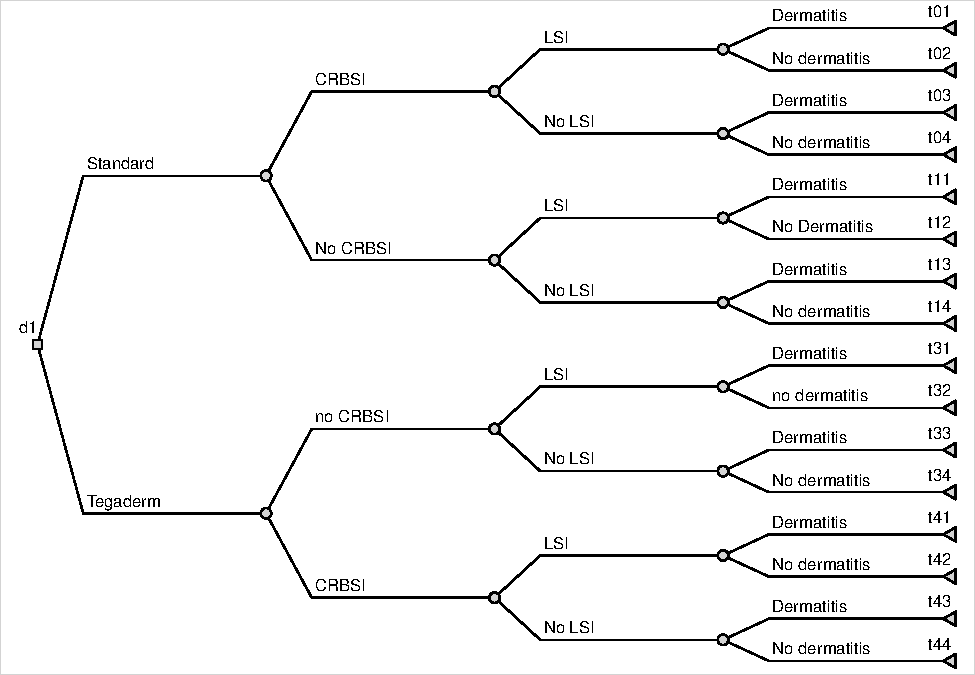
\includegraphics{DT02-Tegaderm_files/figure-latex/draw-1} \end{center}

In the manufacturer's model, the uncertainties in the probabilities
associated with the polytomous chance nodes were modelled as independent
variables. This is not recommended because there is a chance that a
particular run of the PSA will yield probabilities that are outside the
range {[}0,1{]}. Representing the uncertain probabilities with draws
from a Dirichlet distribution is preferred.

\hypertarget{summary-of-the-model}{%
\section{Summary of the model}\label{summary-of-the-model}}

The model variables associated with actions, reactions and leaf nodes
can be tabulated using the method \texttt{modvar\_table}. This returns a
data frame describing each variable, its description, units and
uncertainty distribution. Variables inheriting from type \texttt{ModVar}
will be included in the tabulation; regular numeric values will not be
listed. In the Tegaderm model, the complete structure is as follows:

\begin{longtable}[]{@{}ll@{}}
\toprule
\begin{minipage}[b]{(\columnwidth - 1\tabcolsep) * \real{0.40}}\raggedright
Description\strut
\end{minipage} &
\begin{minipage}[b]{(\columnwidth - 1\tabcolsep) * \real{0.46}}\raggedright
Distribution\strut
\end{minipage}\tabularnewline
\midrule
\endhead
\begin{minipage}[t]{(\columnwidth - 1\tabcolsep) * \real{0.40}}\raggedright
Dermatitis cost\strut
\end{minipage} &
\begin{minipage}[t]{(\columnwidth - 1\tabcolsep) * \real{0.46}}\raggedright
Ga(30,5)\strut
\end{minipage}\tabularnewline
\begin{minipage}[t]{(\columnwidth - 1\tabcolsep) * \real{0.40}}\raggedright
P(dermatitis\textbar standard dressing)\strut
\end{minipage} &
\begin{minipage}[t]{(\columnwidth - 1\tabcolsep) * \real{0.46}}\raggedright
r.Dermatitis * n.catheters\strut
\end{minipage}\tabularnewline
\begin{minipage}[t]{(\columnwidth - 1\tabcolsep) * \real{0.40}}\raggedright
Baseline dermatitis risk\strut
\end{minipage} &
\begin{minipage}[t]{(\columnwidth - 1\tabcolsep) * \real{0.46}}\raggedright
N(0.0026,0.00026)\strut
\end{minipage}\tabularnewline
\begin{minipage}[t]{(\columnwidth - 1\tabcolsep) * \real{0.40}}\raggedright
No.~catheters\strut
\end{minipage} &
\begin{minipage}[t]{(\columnwidth - 1\tabcolsep) * \real{0.46}}\raggedright
N(3,0.3)\strut
\end{minipage}\tabularnewline
\begin{minipage}[t]{(\columnwidth - 1\tabcolsep) * \real{0.40}}\raggedright
Q(dermatitis\textbar standard dressing)\strut
\end{minipage} &
\begin{minipage}[t]{(\columnwidth - 1\tabcolsep) * \real{0.46}}\raggedright
1 - p.Dermatitis.S\strut
\end{minipage}\tabularnewline
\begin{minipage}[t]{(\columnwidth - 1\tabcolsep) * \real{0.40}}\raggedright
LSI cost\strut
\end{minipage} &
\begin{minipage}[t]{(\columnwidth - 1\tabcolsep) * \real{0.46}}\raggedright
Ga(50,5)\strut
\end{minipage}\tabularnewline
\begin{minipage}[t]{(\columnwidth - 1\tabcolsep) * \real{0.40}}\raggedright
P(LSI\textbar Standard)\strut
\end{minipage} &
\begin{minipage}[t]{(\columnwidth - 1\tabcolsep) * \real{0.46}}\raggedright
N(0.1,0.01)\strut
\end{minipage}\tabularnewline
\begin{minipage}[t]{(\columnwidth - 1\tabcolsep) * \real{0.40}}\raggedright
Q(LSI\textbar Standard)\strut
\end{minipage} &
\begin{minipage}[t]{(\columnwidth - 1\tabcolsep) * \real{0.46}}\raggedright
1 - p.LSI.S\strut
\end{minipage}\tabularnewline
\begin{minipage}[t]{(\columnwidth - 1\tabcolsep) * \real{0.40}}\raggedright
CRBSI cost\strut
\end{minipage} &
\begin{minipage}[t]{(\columnwidth - 1\tabcolsep) * \real{0.46}}\raggedright
Ga(198,50)\strut
\end{minipage}\tabularnewline
\begin{minipage}[t]{(\columnwidth - 1\tabcolsep) * \real{0.40}}\raggedright
P(CRBSI\textbar standard dressing)\strut
\end{minipage} &
\begin{minipage}[t]{(\columnwidth - 1\tabcolsep) * \real{0.46}}\raggedright
r.CRBSI * n.cathdays/1000\strut
\end{minipage}\tabularnewline
\begin{minipage}[t]{(\columnwidth - 1\tabcolsep) * \real{0.40}}\raggedright
Baseline CRBSI rate\strut
\end{minipage} &
\begin{minipage}[t]{(\columnwidth - 1\tabcolsep) * \real{0.46}}\raggedright
N(1.48,0.074)\strut
\end{minipage}\tabularnewline
\begin{minipage}[t]{(\columnwidth - 1\tabcolsep) * \real{0.40}}\raggedright
No.~days with catheter\strut
\end{minipage} &
\begin{minipage}[t]{(\columnwidth - 1\tabcolsep) * \real{0.46}}\raggedright
N(10,2)\strut
\end{minipage}\tabularnewline
\begin{minipage}[t]{(\columnwidth - 1\tabcolsep) * \real{0.40}}\raggedright
Q(CRBSI\textbar standard dressing)\strut
\end{minipage} &
\begin{minipage}[t]{(\columnwidth - 1\tabcolsep) * \real{0.46}}\raggedright
1 - p.CRBSI.S\strut
\end{minipage}\tabularnewline
\begin{minipage}[t]{(\columnwidth - 1\tabcolsep) * \real{0.40}}\raggedright
P(dermatitis\textbar Tegaderm)\strut
\end{minipage} &
\begin{minipage}[t]{(\columnwidth - 1\tabcolsep) * \real{0.46}}\raggedright
r.Dermatitis * rr.Dermatitis * n.catheters\strut
\end{minipage}\tabularnewline
\begin{minipage}[t]{(\columnwidth - 1\tabcolsep) * \real{0.40}}\raggedright
Tegaderm LSI HR\strut
\end{minipage} &
\begin{minipage}[t]{(\columnwidth - 1\tabcolsep) * \real{0.46}}\raggedright
exp(1.482 - 0.49 * n3)\strut
\end{minipage}\tabularnewline
\begin{minipage}[t]{(\columnwidth - 1\tabcolsep) * \real{0.40}}\raggedright
SN3\strut
\end{minipage} &
\begin{minipage}[t]{(\columnwidth - 1\tabcolsep) * \real{0.46}}\raggedright
N(0,1)\strut
\end{minipage}\tabularnewline
\begin{minipage}[t]{(\columnwidth - 1\tabcolsep) * \real{0.40}}\raggedright
Q(dermatitis\textbar Tegaderm)\strut
\end{minipage} &
\begin{minipage}[t]{(\columnwidth - 1\tabcolsep) * \real{0.46}}\raggedright
1 - p.Dermatitis.T\strut
\end{minipage}\tabularnewline
\begin{minipage}[t]{(\columnwidth - 1\tabcolsep) * \real{0.40}}\raggedright
P(LSI\textbar Tegaderm)\strut
\end{minipage} &
\begin{minipage}[t]{(\columnwidth - 1\tabcolsep) * \real{0.46}}\raggedright
1 - (1 - p.LSI.S)\^{}hr.LSI\strut
\end{minipage}\tabularnewline
\begin{minipage}[t]{(\columnwidth - 1\tabcolsep) * \real{0.40}}\raggedright
Tegaderm LSI HR\strut
\end{minipage} &
\begin{minipage}[t]{(\columnwidth - 1\tabcolsep) * \real{0.46}}\raggedright
exp(-0.911 - 0.393 * n2)\strut
\end{minipage}\tabularnewline
\begin{minipage}[t]{(\columnwidth - 1\tabcolsep) * \real{0.40}}\raggedright
SN2\strut
\end{minipage} &
\begin{minipage}[t]{(\columnwidth - 1\tabcolsep) * \real{0.46}}\raggedright
N(0,1)\strut
\end{minipage}\tabularnewline
\begin{minipage}[t]{(\columnwidth - 1\tabcolsep) * \real{0.40}}\raggedright
Q(LSI\textbar Tegaderm)\strut
\end{minipage} &
\begin{minipage}[t]{(\columnwidth - 1\tabcolsep) * \real{0.46}}\raggedright
1 - p.LSI.T\strut
\end{minipage}\tabularnewline
\begin{minipage}[t]{(\columnwidth - 1\tabcolsep) * \real{0.40}}\raggedright
P(CRBSI\textbar Tegaderm)\strut
\end{minipage} &
\begin{minipage}[t]{(\columnwidth - 1\tabcolsep) * \real{0.46}}\raggedright
1 - (1 - r.CRBSI * n.cathdays/1000)\^{}hr.CRBSI\strut
\end{minipage}\tabularnewline
\begin{minipage}[t]{(\columnwidth - 1\tabcolsep) * \real{0.40}}\raggedright
Tegaderm CRBSI HR\strut
\end{minipage} &
\begin{minipage}[t]{(\columnwidth - 1\tabcolsep) * \real{0.46}}\raggedright
exp(-0.911 - 0.393 * n1)\strut
\end{minipage}\tabularnewline
\begin{minipage}[t]{(\columnwidth - 1\tabcolsep) * \real{0.40}}\raggedright
SN1\strut
\end{minipage} &
\begin{minipage}[t]{(\columnwidth - 1\tabcolsep) * \real{0.46}}\raggedright
N(0,1)\strut
\end{minipage}\tabularnewline
\begin{minipage}[t]{(\columnwidth - 1\tabcolsep) * \real{0.40}}\raggedright
Q(CRBSI\textbar Tegaderm)\strut
\end{minipage} &
\begin{minipage}[t]{(\columnwidth - 1\tabcolsep) * \real{0.46}}\raggedright
1 - p.CRBSI.T\strut
\end{minipage}\tabularnewline
\begin{minipage}[t]{(\columnwidth - 1\tabcolsep) * \real{0.40}}\raggedright
Standard dressing cost\strut
\end{minipage} &
\begin{minipage}[t]{(\columnwidth - 1\tabcolsep) * \real{0.46}}\raggedright
1.34 * n.catheters\strut
\end{minipage}\tabularnewline
\begin{minipage}[t]{(\columnwidth - 1\tabcolsep) * \real{0.40}}\raggedright
Tegaderm CHG cost\strut
\end{minipage} &
\begin{minipage}[t]{(\columnwidth - 1\tabcolsep) * \real{0.46}}\raggedright
6.21 * n.catheters\strut
\end{minipage}\tabularnewline
\bottomrule
\end{longtable}

\hypertarget{point-estimates-and-distributions-of-model-variables}{%
\section{Point estimates and distributions of model
variables}\label{point-estimates-and-distributions-of-model-variables}}

The point estimates, units and distributional properties are obtained
from the same call, in the remaining columns.

\begin{longtable}[]{@{}lllll@{}}
\toprule
\begin{minipage}[b]{(\columnwidth - 4\tabcolsep) * \real{0.36}}\raggedright
Description\strut
\end{minipage} &
\begin{minipage}[b]{(\columnwidth - 4\tabcolsep) * \real{0.27}}\raggedright
Units\strut
\end{minipage} &
\begin{minipage}[b]{(\columnwidth - 4\tabcolsep) * \real{0.12}}\raggedright
Mean\strut
\end{minipage} &
\begin{minipage}[b]{(\columnwidth - 4\tabcolsep) * \real{0.12}}\raggedright
Q2.5\strut
\end{minipage} &
\begin{minipage}[b]{(\columnwidth - 4\tabcolsep) * \real{0.12}}\raggedright
Q97.5\strut
\end{minipage}\tabularnewline
\midrule
\endhead
\begin{minipage}[t]{(\columnwidth - 4\tabcolsep) * \real{0.36}}\raggedright
Dermatitis cost\strut
\end{minipage} &
\begin{minipage}[t]{(\columnwidth - 4\tabcolsep) * \real{0.27}}\raggedright
GBP\strut
\end{minipage} &
\begin{minipage}[t]{(\columnwidth - 4\tabcolsep) * \real{0.12}}\raggedright
150\strut
\end{minipage} &
\begin{minipage}[t]{(\columnwidth - 4\tabcolsep) * \real{0.12}}\raggedright
101\strut
\end{minipage} &
\begin{minipage}[t]{(\columnwidth - 4\tabcolsep) * \real{0.12}}\raggedright
208\strut
\end{minipage}\tabularnewline
\begin{minipage}[t]{(\columnwidth - 4\tabcolsep) * \real{0.36}}\raggedright
P(dermatitis\textbar standard dressing)\strut
\end{minipage} &
\begin{minipage}[t]{(\columnwidth - 4\tabcolsep) * \real{0.27}}\raggedright
P\strut
\end{minipage} &
\begin{minipage}[t]{(\columnwidth - 4\tabcolsep) * \real{0.12}}\raggedright
0.0078\strut
\end{minipage} &
\begin{minipage}[t]{(\columnwidth - 4\tabcolsep) * \real{0.12}}\raggedright
0.0058\strut
\end{minipage} &
\begin{minipage}[t]{(\columnwidth - 4\tabcolsep) * \real{0.12}}\raggedright
0.0102\strut
\end{minipage}\tabularnewline
\begin{minipage}[t]{(\columnwidth - 4\tabcolsep) * \real{0.36}}\raggedright
Baseline dermatitis risk\strut
\end{minipage} &
\begin{minipage}[t]{(\columnwidth - 4\tabcolsep) * \real{0.27}}\raggedright
/catheter\strut
\end{minipage} &
\begin{minipage}[t]{(\columnwidth - 4\tabcolsep) * \real{0.12}}\raggedright
0.0026\strut
\end{minipage} &
\begin{minipage}[t]{(\columnwidth - 4\tabcolsep) * \real{0.12}}\raggedright
0.00209\strut
\end{minipage} &
\begin{minipage}[t]{(\columnwidth - 4\tabcolsep) * \real{0.12}}\raggedright
0.00311\strut
\end{minipage}\tabularnewline
\begin{minipage}[t]{(\columnwidth - 4\tabcolsep) * \real{0.36}}\raggedright
No.~catheters\strut
\end{minipage} &
\begin{minipage}[t]{(\columnwidth - 4\tabcolsep) * \real{0.27}}\raggedright
catheters\strut
\end{minipage} &
\begin{minipage}[t]{(\columnwidth - 4\tabcolsep) * \real{0.12}}\raggedright
3\strut
\end{minipage} &
\begin{minipage}[t]{(\columnwidth - 4\tabcolsep) * \real{0.12}}\raggedright
2.41\strut
\end{minipage} &
\begin{minipage}[t]{(\columnwidth - 4\tabcolsep) * \real{0.12}}\raggedright
3.59\strut
\end{minipage}\tabularnewline
\begin{minipage}[t]{(\columnwidth - 4\tabcolsep) * \real{0.36}}\raggedright
Q(dermatitis\textbar standard dressing)\strut
\end{minipage} &
\begin{minipage}[t]{(\columnwidth - 4\tabcolsep) * \real{0.27}}\raggedright
1-P\strut
\end{minipage} &
\begin{minipage}[t]{(\columnwidth - 4\tabcolsep) * \real{0.12}}\raggedright
0.992\strut
\end{minipage} &
\begin{minipage}[t]{(\columnwidth - 4\tabcolsep) * \real{0.12}}\raggedright
0.99\strut
\end{minipage} &
\begin{minipage}[t]{(\columnwidth - 4\tabcolsep) * \real{0.12}}\raggedright
0.994\strut
\end{minipage}\tabularnewline
\begin{minipage}[t]{(\columnwidth - 4\tabcolsep) * \real{0.36}}\raggedright
LSI cost\strut
\end{minipage} &
\begin{minipage}[t]{(\columnwidth - 4\tabcolsep) * \real{0.27}}\raggedright
GBP\strut
\end{minipage} &
\begin{minipage}[t]{(\columnwidth - 4\tabcolsep) * \real{0.12}}\raggedright
250\strut
\end{minipage} &
\begin{minipage}[t]{(\columnwidth - 4\tabcolsep) * \real{0.12}}\raggedright
186\strut
\end{minipage} &
\begin{minipage}[t]{(\columnwidth - 4\tabcolsep) * \real{0.12}}\raggedright
324\strut
\end{minipage}\tabularnewline
\begin{minipage}[t]{(\columnwidth - 4\tabcolsep) * \real{0.36}}\raggedright
P(LSI\textbar Standard)\strut
\end{minipage} &
\begin{minipage}[t]{(\columnwidth - 4\tabcolsep) * \real{0.27}}\raggedright
/patient\strut
\end{minipage} &
\begin{minipage}[t]{(\columnwidth - 4\tabcolsep) * \real{0.12}}\raggedright
0.1\strut
\end{minipage} &
\begin{minipage}[t]{(\columnwidth - 4\tabcolsep) * \real{0.12}}\raggedright
0.0804\strut
\end{minipage} &
\begin{minipage}[t]{(\columnwidth - 4\tabcolsep) * \real{0.12}}\raggedright
0.12\strut
\end{minipage}\tabularnewline
\begin{minipage}[t]{(\columnwidth - 4\tabcolsep) * \real{0.36}}\raggedright
Q(LSI\textbar Standard)\strut
\end{minipage} &
\begin{minipage}[t]{(\columnwidth - 4\tabcolsep) * \real{0.27}}\raggedright
1-P\strut
\end{minipage} &
\begin{minipage}[t]{(\columnwidth - 4\tabcolsep) * \real{0.12}}\raggedright
0.9\strut
\end{minipage} &
\begin{minipage}[t]{(\columnwidth - 4\tabcolsep) * \real{0.12}}\raggedright
0.88\strut
\end{minipage} &
\begin{minipage}[t]{(\columnwidth - 4\tabcolsep) * \real{0.12}}\raggedright
0.92\strut
\end{minipage}\tabularnewline
\begin{minipage}[t]{(\columnwidth - 4\tabcolsep) * \real{0.36}}\raggedright
CRBSI cost\strut
\end{minipage} &
\begin{minipage}[t]{(\columnwidth - 4\tabcolsep) * \real{0.27}}\raggedright
GBP\strut
\end{minipage} &
\begin{minipage}[t]{(\columnwidth - 4\tabcolsep) * \real{0.12}}\raggedright
9900\strut
\end{minipage} &
\begin{minipage}[t]{(\columnwidth - 4\tabcolsep) * \real{0.12}}\raggedright
8569\strut
\end{minipage} &
\begin{minipage}[t]{(\columnwidth - 4\tabcolsep) * \real{0.12}}\raggedright
11326\strut
\end{minipage}\tabularnewline
\begin{minipage}[t]{(\columnwidth - 4\tabcolsep) * \real{0.36}}\raggedright
P(CRBSI\textbar standard dressing)\strut
\end{minipage} &
\begin{minipage}[t]{(\columnwidth - 4\tabcolsep) * \real{0.27}}\raggedright
P\strut
\end{minipage} &
\begin{minipage}[t]{(\columnwidth - 4\tabcolsep) * \real{0.12}}\raggedright
0.0148\strut
\end{minipage} &
\begin{minipage}[t]{(\columnwidth - 4\tabcolsep) * \real{0.12}}\raggedright
0.00908\strut
\end{minipage} &
\begin{minipage}[t]{(\columnwidth - 4\tabcolsep) * \real{0.12}}\raggedright
0.021\strut
\end{minipage}\tabularnewline
\begin{minipage}[t]{(\columnwidth - 4\tabcolsep) * \real{0.36}}\raggedright
Baseline CRBSI rate\strut
\end{minipage} &
\begin{minipage}[t]{(\columnwidth - 4\tabcolsep) * \real{0.27}}\raggedright
/1000 catheter days\strut
\end{minipage} &
\begin{minipage}[t]{(\columnwidth - 4\tabcolsep) * \real{0.12}}\raggedright
1.48\strut
\end{minipage} &
\begin{minipage}[t]{(\columnwidth - 4\tabcolsep) * \real{0.12}}\raggedright
1.33\strut
\end{minipage} &
\begin{minipage}[t]{(\columnwidth - 4\tabcolsep) * \real{0.12}}\raggedright
1.63\strut
\end{minipage}\tabularnewline
\begin{minipage}[t]{(\columnwidth - 4\tabcolsep) * \real{0.36}}\raggedright
No.~days with catheter\strut
\end{minipage} &
\begin{minipage}[t]{(\columnwidth - 4\tabcolsep) * \real{0.27}}\raggedright
days\strut
\end{minipage} &
\begin{minipage}[t]{(\columnwidth - 4\tabcolsep) * \real{0.12}}\raggedright
10\strut
\end{minipage} &
\begin{minipage}[t]{(\columnwidth - 4\tabcolsep) * \real{0.12}}\raggedright
6.08\strut
\end{minipage} &
\begin{minipage}[t]{(\columnwidth - 4\tabcolsep) * \real{0.12}}\raggedright
13.9\strut
\end{minipage}\tabularnewline
\begin{minipage}[t]{(\columnwidth - 4\tabcolsep) * \real{0.36}}\raggedright
Q(CRBSI\textbar standard dressing)\strut
\end{minipage} &
\begin{minipage}[t]{(\columnwidth - 4\tabcolsep) * \real{0.27}}\raggedright
1-P\strut
\end{minipage} &
\begin{minipage}[t]{(\columnwidth - 4\tabcolsep) * \real{0.12}}\raggedright
0.985\strut
\end{minipage} &
\begin{minipage}[t]{(\columnwidth - 4\tabcolsep) * \real{0.12}}\raggedright
0.979\strut
\end{minipage} &
\begin{minipage}[t]{(\columnwidth - 4\tabcolsep) * \real{0.12}}\raggedright
0.992\strut
\end{minipage}\tabularnewline
\begin{minipage}[t]{(\columnwidth - 4\tabcolsep) * \real{0.36}}\raggedright
P(dermatitis\textbar Tegaderm)\strut
\end{minipage} &
\begin{minipage}[t]{(\columnwidth - 4\tabcolsep) * \real{0.27}}\raggedright
P\strut
\end{minipage} &
\begin{minipage}[t]{(\columnwidth - 4\tabcolsep) * \real{0.12}}\raggedright
0.0343\strut
\end{minipage} &
\begin{minipage}[t]{(\columnwidth - 4\tabcolsep) * \real{0.12}}\raggedright
0.0132\strut
\end{minipage} &
\begin{minipage}[t]{(\columnwidth - 4\tabcolsep) * \real{0.12}}\raggedright
0.0932\strut
\end{minipage}\tabularnewline
\begin{minipage}[t]{(\columnwidth - 4\tabcolsep) * \real{0.36}}\raggedright
Tegaderm LSI HR\strut
\end{minipage} &
\begin{minipage}[t]{(\columnwidth - 4\tabcolsep) * \real{0.27}}\raggedright
HR\strut
\end{minipage} &
\begin{minipage}[t]{(\columnwidth - 4\tabcolsep) * \real{0.12}}\raggedright
4.4\strut
\end{minipage} &
\begin{minipage}[t]{(\columnwidth - 4\tabcolsep) * \real{0.12}}\raggedright
1.65\strut
\end{minipage} &
\begin{minipage}[t]{(\columnwidth - 4\tabcolsep) * \real{0.12}}\raggedright
12.1\strut
\end{minipage}\tabularnewline
\begin{minipage}[t]{(\columnwidth - 4\tabcolsep) * \real{0.36}}\raggedright
SN3\strut
\end{minipage} &
\begin{minipage}[t]{(\columnwidth - 4\tabcolsep) * \real{0.27}}\raggedright
\strut
\end{minipage} &
\begin{minipage}[t]{(\columnwidth - 4\tabcolsep) * \real{0.12}}\raggedright
0\strut
\end{minipage} &
\begin{minipage}[t]{(\columnwidth - 4\tabcolsep) * \real{0.12}}\raggedright
-1.96\strut
\end{minipage} &
\begin{minipage}[t]{(\columnwidth - 4\tabcolsep) * \real{0.12}}\raggedright
1.96\strut
\end{minipage}\tabularnewline
\begin{minipage}[t]{(\columnwidth - 4\tabcolsep) * \real{0.36}}\raggedright
Q(dermatitis\textbar Tegaderm)\strut
\end{minipage} &
\begin{minipage}[t]{(\columnwidth - 4\tabcolsep) * \real{0.27}}\raggedright
1-P\strut
\end{minipage} &
\begin{minipage}[t]{(\columnwidth - 4\tabcolsep) * \real{0.12}}\raggedright
0.966\strut
\end{minipage} &
\begin{minipage}[t]{(\columnwidth - 4\tabcolsep) * \real{0.12}}\raggedright
0.907\strut
\end{minipage} &
\begin{minipage}[t]{(\columnwidth - 4\tabcolsep) * \real{0.12}}\raggedright
0.988\strut
\end{minipage}\tabularnewline
\begin{minipage}[t]{(\columnwidth - 4\tabcolsep) * \real{0.36}}\raggedright
P(LSI\textbar Tegaderm)\strut
\end{minipage} &
\begin{minipage}[t]{(\columnwidth - 4\tabcolsep) * \real{0.27}}\raggedright
P\strut
\end{minipage} &
\begin{minipage}[t]{(\columnwidth - 4\tabcolsep) * \real{0.12}}\raggedright
0.0415\strut
\end{minipage} &
\begin{minipage}[t]{(\columnwidth - 4\tabcolsep) * \real{0.12}}\raggedright
0.0178\strut
\end{minipage} &
\begin{minipage}[t]{(\columnwidth - 4\tabcolsep) * \real{0.12}}\raggedright
0.0842\strut
\end{minipage}\tabularnewline
\begin{minipage}[t]{(\columnwidth - 4\tabcolsep) * \real{0.36}}\raggedright
Tegaderm LSI HR\strut
\end{minipage} &
\begin{minipage}[t]{(\columnwidth - 4\tabcolsep) * \real{0.27}}\raggedright
HR\strut
\end{minipage} &
\begin{minipage}[t]{(\columnwidth - 4\tabcolsep) * \real{0.12}}\raggedright
0.402\strut
\end{minipage} &
\begin{minipage}[t]{(\columnwidth - 4\tabcolsep) * \real{0.12}}\raggedright
0.183\strut
\end{minipage} &
\begin{minipage}[t]{(\columnwidth - 4\tabcolsep) * \real{0.12}}\raggedright
0.867\strut
\end{minipage}\tabularnewline
\begin{minipage}[t]{(\columnwidth - 4\tabcolsep) * \real{0.36}}\raggedright
SN2\strut
\end{minipage} &
\begin{minipage}[t]{(\columnwidth - 4\tabcolsep) * \real{0.27}}\raggedright
\strut
\end{minipage} &
\begin{minipage}[t]{(\columnwidth - 4\tabcolsep) * \real{0.12}}\raggedright
0\strut
\end{minipage} &
\begin{minipage}[t]{(\columnwidth - 4\tabcolsep) * \real{0.12}}\raggedright
-1.96\strut
\end{minipage} &
\begin{minipage}[t]{(\columnwidth - 4\tabcolsep) * \real{0.12}}\raggedright
1.96\strut
\end{minipage}\tabularnewline
\begin{minipage}[t]{(\columnwidth - 4\tabcolsep) * \real{0.36}}\raggedright
Q(LSI\textbar Tegaderm)\strut
\end{minipage} &
\begin{minipage}[t]{(\columnwidth - 4\tabcolsep) * \real{0.27}}\raggedright
1-P\strut
\end{minipage} &
\begin{minipage}[t]{(\columnwidth - 4\tabcolsep) * \real{0.12}}\raggedright
0.959\strut
\end{minipage} &
\begin{minipage}[t]{(\columnwidth - 4\tabcolsep) * \real{0.12}}\raggedright
0.911\strut
\end{minipage} &
\begin{minipage}[t]{(\columnwidth - 4\tabcolsep) * \real{0.12}}\raggedright
0.981\strut
\end{minipage}\tabularnewline
\begin{minipage}[t]{(\columnwidth - 4\tabcolsep) * \real{0.36}}\raggedright
P(CRBSI\textbar Tegaderm)\strut
\end{minipage} &
\begin{minipage}[t]{(\columnwidth - 4\tabcolsep) * \real{0.27}}\raggedright
P\strut
\end{minipage} &
\begin{minipage}[t]{(\columnwidth - 4\tabcolsep) * \real{0.12}}\raggedright
0.00598\strut
\end{minipage} &
\begin{minipage}[t]{(\columnwidth - 4\tabcolsep) * \real{0.12}}\raggedright
0.00234\strut
\end{minipage} &
\begin{minipage}[t]{(\columnwidth - 4\tabcolsep) * \real{0.12}}\raggedright
0.0136\strut
\end{minipage}\tabularnewline
\begin{minipage}[t]{(\columnwidth - 4\tabcolsep) * \real{0.36}}\raggedright
Tegaderm CRBSI HR\strut
\end{minipage} &
\begin{minipage}[t]{(\columnwidth - 4\tabcolsep) * \real{0.27}}\raggedright
HR\strut
\end{minipage} &
\begin{minipage}[t]{(\columnwidth - 4\tabcolsep) * \real{0.12}}\raggedright
0.402\strut
\end{minipage} &
\begin{minipage}[t]{(\columnwidth - 4\tabcolsep) * \real{0.12}}\raggedright
0.185\strut
\end{minipage} &
\begin{minipage}[t]{(\columnwidth - 4\tabcolsep) * \real{0.12}}\raggedright
0.851\strut
\end{minipage}\tabularnewline
\begin{minipage}[t]{(\columnwidth - 4\tabcolsep) * \real{0.36}}\raggedright
SN1\strut
\end{minipage} &
\begin{minipage}[t]{(\columnwidth - 4\tabcolsep) * \real{0.27}}\raggedright
\strut
\end{minipage} &
\begin{minipage}[t]{(\columnwidth - 4\tabcolsep) * \real{0.12}}\raggedright
0\strut
\end{minipage} &
\begin{minipage}[t]{(\columnwidth - 4\tabcolsep) * \real{0.12}}\raggedright
-1.96\strut
\end{minipage} &
\begin{minipage}[t]{(\columnwidth - 4\tabcolsep) * \real{0.12}}\raggedright
1.96\strut
\end{minipage}\tabularnewline
\begin{minipage}[t]{(\columnwidth - 4\tabcolsep) * \real{0.36}}\raggedright
Q(CRBSI\textbar Tegaderm)\strut
\end{minipage} &
\begin{minipage}[t]{(\columnwidth - 4\tabcolsep) * \real{0.27}}\raggedright
1-P\strut
\end{minipage} &
\begin{minipage}[t]{(\columnwidth - 4\tabcolsep) * \real{0.12}}\raggedright
0.994\strut
\end{minipage} &
\begin{minipage}[t]{(\columnwidth - 4\tabcolsep) * \real{0.12}}\raggedright
0.986\strut
\end{minipage} &
\begin{minipage}[t]{(\columnwidth - 4\tabcolsep) * \real{0.12}}\raggedright
0.998\strut
\end{minipage}\tabularnewline
\begin{minipage}[t]{(\columnwidth - 4\tabcolsep) * \real{0.36}}\raggedright
Standard dressing cost\strut
\end{minipage} &
\begin{minipage}[t]{(\columnwidth - 4\tabcolsep) * \real{0.27}}\raggedright
GBP\strut
\end{minipage} &
\begin{minipage}[t]{(\columnwidth - 4\tabcolsep) * \real{0.12}}\raggedright
4.02\strut
\end{minipage} &
\begin{minipage}[t]{(\columnwidth - 4\tabcolsep) * \real{0.12}}\raggedright
3.23\strut
\end{minipage} &
\begin{minipage}[t]{(\columnwidth - 4\tabcolsep) * \real{0.12}}\raggedright
4.83\strut
\end{minipage}\tabularnewline
\begin{minipage}[t]{(\columnwidth - 4\tabcolsep) * \real{0.36}}\raggedright
Tegaderm CHG cost\strut
\end{minipage} &
\begin{minipage}[t]{(\columnwidth - 4\tabcolsep) * \real{0.27}}\raggedright
GBP\strut
\end{minipage} &
\begin{minipage}[t]{(\columnwidth - 4\tabcolsep) * \real{0.12}}\raggedright
18.6\strut
\end{minipage} &
\begin{minipage}[t]{(\columnwidth - 4\tabcolsep) * \real{0.12}}\raggedright
15\strut
\end{minipage} &
\begin{minipage}[t]{(\columnwidth - 4\tabcolsep) * \real{0.12}}\raggedright
22.2\strut
\end{minipage}\tabularnewline
\bottomrule
\end{longtable}

\hypertarget{running-the-model-base-case}{%
\section{Running the model: base
case}\label{running-the-model-base-case}}

The following code runs a single model scenario, using the
\texttt{evaluate} method of a decision node to evaluate each pathway
from the decision node, shown in the table. This model did not consider
utility, and the columns associated with utility are removed.

\begin{Shaded}
\begin{Highlighting}[]
\NormalTok{RES }\OtherTok{\textless{}{-}}\NormalTok{ DT}\SpecialCharTok{$}\FunctionTok{evaluate}\NormalTok{()}
\end{Highlighting}
\end{Shaded}

\begin{longtable}[]{@{}llr@{}}
\toprule
\begin{minipage}[b]{(\columnwidth - 2\tabcolsep) * \real{0.08}}\raggedright
Run\strut
\end{minipage} &
\begin{minipage}[b]{(\columnwidth - 2\tabcolsep) * \real{0.15}}\raggedright
d1\strut
\end{minipage} &
\begin{minipage}[b]{(\columnwidth - 2\tabcolsep) * \real{0.11}}\raggedleft
Cost\strut
\end{minipage}\tabularnewline
\midrule
\endhead
\begin{minipage}[t]{(\columnwidth - 2\tabcolsep) * \real{0.08}}\raggedright
1\strut
\end{minipage} &
\begin{minipage}[t]{(\columnwidth - 2\tabcolsep) * \real{0.15}}\raggedright
Standard\strut
\end{minipage} &
\begin{minipage}[t]{(\columnwidth - 2\tabcolsep) * \real{0.11}}\raggedleft
176.7\strut
\end{minipage}\tabularnewline
\begin{minipage}[t]{(\columnwidth - 2\tabcolsep) * \real{0.08}}\raggedright
1\strut
\end{minipage} &
\begin{minipage}[t]{(\columnwidth - 2\tabcolsep) * \real{0.15}}\raggedright
Tegaderm\strut
\end{minipage} &
\begin{minipage}[t]{(\columnwidth - 2\tabcolsep) * \real{0.11}}\raggedleft
93.33\strut
\end{minipage}\tabularnewline
\bottomrule
\end{longtable}

\hypertarget{running-the-model-probabilistic-sensitivity-analysis}{%
\section{Running the model: probabilistic sensitivity
analysis}\label{running-the-model-probabilistic-sensitivity-analysis}}

Probabilistic sensitivity analysis is supported through the use of
sampling model variables. The same call, with extra parameters is used
to run the PSA:

\begin{Shaded}
\begin{Highlighting}[]
\NormalTok{PSA }\OtherTok{\textless{}{-}}\NormalTok{ DT}\SpecialCharTok{$}\FunctionTok{evaluate}\NormalTok{(}\AttributeTok{expected=}\NormalTok{F, }\AttributeTok{N=}\DecValTok{100}\NormalTok{)}
\end{Highlighting}
\end{Shaded}

The first few runs of PSA are as follows (after reshaping the table to
give one row per simulation, rather than one row per run, per strategy):

\begin{longtable}[]{@{}lrrr@{}}
\toprule
\begin{minipage}[b]{(\columnwidth - 3\tabcolsep) * \real{0.08}}\raggedright
Run\strut
\end{minipage} &
\begin{minipage}[b]{(\columnwidth - 3\tabcolsep) * \real{0.22}}\raggedleft
Cost.Tegaderm\strut
\end{minipage} &
\begin{minipage}[b]{(\columnwidth - 3\tabcolsep) * \real{0.22}}\raggedleft
Cost.Standard\strut
\end{minipage} &
\begin{minipage}[b]{(\columnwidth - 3\tabcolsep) * \real{0.18}}\raggedleft
Difference\strut
\end{minipage}\tabularnewline
\midrule
\endhead
\begin{minipage}[t]{(\columnwidth - 3\tabcolsep) * \real{0.08}}\raggedright
1\strut
\end{minipage} &
\begin{minipage}[t]{(\columnwidth - 3\tabcolsep) * \real{0.22}}\raggedleft
118.5\strut
\end{minipage} &
\begin{minipage}[t]{(\columnwidth - 3\tabcolsep) * \real{0.22}}\raggedleft
197.3\strut
\end{minipage} &
\begin{minipage}[t]{(\columnwidth - 3\tabcolsep) * \real{0.18}}\raggedleft
-78.79\strut
\end{minipage}\tabularnewline
\begin{minipage}[t]{(\columnwidth - 3\tabcolsep) * \real{0.08}}\raggedright
2\strut
\end{minipage} &
\begin{minipage}[t]{(\columnwidth - 3\tabcolsep) * \real{0.22}}\raggedleft
120.6\strut
\end{minipage} &
\begin{minipage}[t]{(\columnwidth - 3\tabcolsep) * \real{0.22}}\raggedleft
179.4\strut
\end{minipage} &
\begin{minipage}[t]{(\columnwidth - 3\tabcolsep) * \real{0.18}}\raggedleft
-58.73\strut
\end{minipage}\tabularnewline
\begin{minipage}[t]{(\columnwidth - 3\tabcolsep) * \real{0.08}}\raggedright
3\strut
\end{minipage} &
\begin{minipage}[t]{(\columnwidth - 3\tabcolsep) * \real{0.22}}\raggedleft
77.52\strut
\end{minipage} &
\begin{minipage}[t]{(\columnwidth - 3\tabcolsep) * \real{0.22}}\raggedleft
184.5\strut
\end{minipage} &
\begin{minipage}[t]{(\columnwidth - 3\tabcolsep) * \real{0.18}}\raggedleft
-107\strut
\end{minipage}\tabularnewline
\begin{minipage}[t]{(\columnwidth - 3\tabcolsep) * \real{0.08}}\raggedright
4\strut
\end{minipage} &
\begin{minipage}[t]{(\columnwidth - 3\tabcolsep) * \real{0.22}}\raggedleft
130.5\strut
\end{minipage} &
\begin{minipage}[t]{(\columnwidth - 3\tabcolsep) * \real{0.22}}\raggedleft
208\strut
\end{minipage} &
\begin{minipage}[t]{(\columnwidth - 3\tabcolsep) * \real{0.18}}\raggedleft
-77.46\strut
\end{minipage}\tabularnewline
\begin{minipage}[t]{(\columnwidth - 3\tabcolsep) * \real{0.08}}\raggedright
5\strut
\end{minipage} &
\begin{minipage}[t]{(\columnwidth - 3\tabcolsep) * \real{0.22}}\raggedleft
171.8\strut
\end{minipage} &
\begin{minipage}[t]{(\columnwidth - 3\tabcolsep) * \real{0.22}}\raggedleft
194.8\strut
\end{minipage} &
\begin{minipage}[t]{(\columnwidth - 3\tabcolsep) * \real{0.18}}\raggedleft
-23.04\strut
\end{minipage}\tabularnewline
\begin{minipage}[t]{(\columnwidth - 3\tabcolsep) * \real{0.08}}\raggedright
6\strut
\end{minipage} &
\begin{minipage}[t]{(\columnwidth - 3\tabcolsep) * \real{0.22}}\raggedleft
111.4\strut
\end{minipage} &
\begin{minipage}[t]{(\columnwidth - 3\tabcolsep) * \real{0.22}}\raggedleft
190.3\strut
\end{minipage} &
\begin{minipage}[t]{(\columnwidth - 3\tabcolsep) * \real{0.18}}\raggedleft
-78.95\strut
\end{minipage}\tabularnewline
\begin{minipage}[t]{(\columnwidth - 3\tabcolsep) * \real{0.08}}\raggedright
7\strut
\end{minipage} &
\begin{minipage}[t]{(\columnwidth - 3\tabcolsep) * \real{0.22}}\raggedleft
97.74\strut
\end{minipage} &
\begin{minipage}[t]{(\columnwidth - 3\tabcolsep) * \real{0.22}}\raggedleft
215.1\strut
\end{minipage} &
\begin{minipage}[t]{(\columnwidth - 3\tabcolsep) * \real{0.18}}\raggedleft
-117.4\strut
\end{minipage}\tabularnewline
\begin{minipage}[t]{(\columnwidth - 3\tabcolsep) * \real{0.08}}\raggedright
8\strut
\end{minipage} &
\begin{minipage}[t]{(\columnwidth - 3\tabcolsep) * \real{0.22}}\raggedleft
118.3\strut
\end{minipage} &
\begin{minipage}[t]{(\columnwidth - 3\tabcolsep) * \real{0.22}}\raggedleft
167.7\strut
\end{minipage} &
\begin{minipage}[t]{(\columnwidth - 3\tabcolsep) * \real{0.18}}\raggedleft
-49.47\strut
\end{minipage}\tabularnewline
\begin{minipage}[t]{(\columnwidth - 3\tabcolsep) * \real{0.08}}\raggedright
9\strut
\end{minipage} &
\begin{minipage}[t]{(\columnwidth - 3\tabcolsep) * \real{0.22}}\raggedleft
76.45\strut
\end{minipage} &
\begin{minipage}[t]{(\columnwidth - 3\tabcolsep) * \real{0.22}}\raggedleft
155.9\strut
\end{minipage} &
\begin{minipage}[t]{(\columnwidth - 3\tabcolsep) * \real{0.18}}\raggedleft
-79.49\strut
\end{minipage}\tabularnewline
\begin{minipage}[t]{(\columnwidth - 3\tabcolsep) * \real{0.08}}\raggedright
10\strut
\end{minipage} &
\begin{minipage}[t]{(\columnwidth - 3\tabcolsep) * \real{0.22}}\raggedleft
85.34\strut
\end{minipage} &
\begin{minipage}[t]{(\columnwidth - 3\tabcolsep) * \real{0.22}}\raggedleft
149.8\strut
\end{minipage} &
\begin{minipage}[t]{(\columnwidth - 3\tabcolsep) * \real{0.18}}\raggedleft
-64.41\strut
\end{minipage}\tabularnewline
\bottomrule
\end{longtable}

From PSA (100 runs), the mean cost of treatment with Tegaderm was
104.41, the mean cost of treatment with standard dressings was 181.37
and the mean cost saving was -76.96. The 95\% confidence interval for
cost saving was -137.11 to -14.99; the standard deviation of the cost
saving was 30.53. Overall, 100\% of runs found that Tegaderm was cost
saving. These results replicate those reported by the manufacturer
(saving of 77.76, 98.5\% cases cost saving; mean cost of standard
dressing 176.89, mean cost of Tegaderm 99.63).

\hypertarget{references}{%
\section*{References}\label{references}}
\addcontentsline{toc}{section}{References}

\hypertarget{refs}{}
\begin{CSLReferences}{0}{0}
\leavevmode\hypertarget{ref-jenks2016}{}%
\CSLLeftMargin{1 }
\CSLRightInline{Jenks M, Craig J, Green W, \emph{et al.} Tegaderm {CHG}
{IV} securement dressing for central venous and arterial catheter
insertion sites: A {NICE} medical technology guidance. \emph{Applied
Health Economics and Health Policy} 2016;\textbf{14}:135--49.
doi:\href{https://doi.org/10.1007/s40258-015-0202-5}{10.1007/s40258-015-0202-5}}

\leavevmode\hypertarget{ref-briggs2006}{}%
\CSLLeftMargin{2 }
\CSLRightInline{Briggs A, Claxton K, Sculpher M. \emph{Decision
modelling for health economic evaluation}. Oxford, {UK}: : Oxford
University Press 2006. }

\end{CSLReferences}

\end{document}
